\documentclass[12pt,a4paper]{report}

\usepackage[a4paper,margin=1in]{geometry}
\usepackage{iftex}
\ifPDFTeX
  \usepackage[T1]{fontenc}
  \usepackage[utf8]{inputenc}
  \usepackage{newtxtext,newtxmath}
\else
  \usepackage{fontspec}
  \setmainfont{Times New Roman}
\fi
\usepackage{setspace}
\onehalfspacing
\usepackage{graphicx}
\usepackage{titlesec}
\usepackage{fancyhdr}
\usepackage{hyperref}
\usepackage{longtable}
\usepackage{booktabs}
\usepackage{array}
\usepackage{enumitem}
\usepackage{caption}
\usepackage{tikz}
\usetikzlibrary{positioning,arrows.meta}
\usepackage{float}
\usepackage{ragged2e}
\usepackage{tocloft}
\usepackage{xcolor}

\hypersetup{
    colorlinks=true,
    linkcolor=black,
    urlcolor=blue,
    citecolor=black
}

\setlength{\parindent}{0.5in}
\setlength{\parskip}{0pt}
\justifying

% -------------------------
% Editable project details
% -------------------------
\newcommand{\UniversityName}{SAVITRIBAI PHULE PUNE UNIVERSITY}
\newcommand{\CollegeName}{AMRUTVAHINI COLLEGE OF ENGINEERING, SANGAMNER-422608}
\newcommand{\CollegeNameShort}{AMRUTVAHINI COLLEGE OF ENGINEERING, SANGAMNER}
\newcommand{\DepartmentName}{DEPARTMENT OF COMPUTER ENGINEERING}
\newcommand{\ProjectTitle}{Ebook Shop}
\newcommand{\StudentOneName}{Aditya Bhausaheb Akolkar}
\newcommand{\StudentOneRoll}{4503}
\newcommand{\StudentTwoName}{Sai Shyam Abhang}
\newcommand{\StudentTwoRoll}{4501}
\newcommand{\GuideName}{Prof. Y. A. Shinde}
\newcommand{\AcademicYear}{2025-2026}
\newcommand{\CourseName}{Web Technology Laboratory (WTL)}
\newcommand{\ClassName}{T.E. Computer Engineering}
\newcommand{\DegreeName}{Bachelor of Engineering}
\newcommand{\SemesterName}{SEM-II}

\begin{document}
\pagenumbering{gobble}

% ==================================================
% PAGE 1 — TITLE PAGE
% ==================================================
\begin{titlepage}
    \centering

    {\Large\bfseries \UniversityName \par}
    \vspace{1.2cm}

    {\Large Mini Project Report On \par}
    \vspace{0.7cm}

    {\Huge\bfseries ``\ProjectTitle'' \par}
    \vspace{1.0cm}

    {\large SUBMITTED TO THE SAVITRIBAI PHULE PUNE UNIVERSITY, PUNE \par}
    \vspace{0.25cm}
    {\large IN THE PARTIAL FULFILLMENT OF THE REQUIREMENT \par}
    {\large FOR THE \ClassName \par}
    {\large \DegreeName \par}
    {\large (Computer Engineering) (\SemesterName) \par}

    \vspace{1.1cm}
    {\large SUBMITTED BY \par}
    \vspace{0.3cm}
    {\large \StudentOneName\ (\StudentOneRoll) \par}
    {\large \StudentTwoName\ (\StudentTwoRoll) \par}

    \vspace{0.9cm}
    {\large UNDER THE GUIDANCE OF \par}
    \vspace{0.3cm}
    {\large \GuideName \par}

    \vspace{0.9cm}
    {\large DURING THE ACADEMIC YEAR \AcademicYear \par}

    \vfill

    {\large\bfseries \DepartmentName \par}
    {\large\bfseries AMRUTVAHINI COLLEGE OF ENGINEERING, SANGAMNER-422608 \par}
    {\large\bfseries ACADEMIC YEAR \AcademicYear \par}

\end{titlepage}

% ==================================================
% PAGE 2 — CERTIFICATE
% ==================================================
\clearpage
\thispagestyle{empty}

\begin{center}
    {\large\bfseries AMRUTVAHINI COLLEGE OF ENGINEERING, SANGAMNER \par}
    {\large\bfseries DEPARTMENT OF COMPUTER ENGINEERING \par}
    \vspace{0.9cm}
    {\Large\bfseries CERTIFICATE \par}
\end{center}

\vspace{0.9cm}

\noindent
This is to certify that,\\[0.4cm]
\StudentOneName\ and \StudentTwoName\ students in Third Year Division A, Computer Engineering has successfully completed their Mini Project titled ``\ProjectTitle'' at Amrutvahini College of Engineering, Sangamner.

\vspace{0.4cm}

\noindent
This project work is submitted in partial fulfillment of the requirements for the subject \CourseName\ of the Third Year Bachelor of Engineering in Computer Engineering during the academic year \AcademicYear.

\vspace{2.5cm}

\begin{flushright}
\GuideName\\
Coordinator
\end{flushright}

% ==================================================
% PAGE 3 — CONTENTS
% ==================================================
\clearpage
\thispagestyle{empty}
\tableofcontents
\clearpage

\setcounter{page}{1}
\pagenumbering{arabic}

\chapter{Introduction}
Ebook Shop is a web-based mini project developed as a full-stack academic application for digital book browsing and ordering. The frontend is implemented using React and Vite, while the backend is implemented using Express and MongoDB through Mongoose schemas. The project demonstrates practical web engineering concepts such as routing, token-based authentication, shared state management, database integration, and REST API communication.

The project addresses a common student-level problem: available learning resources are scattered across multiple platforms, and beginners require a single interface where they can browse category-wise ebooks, compare options, maintain a wishlist, and complete checkout in a structured flow. Ebook Shop organizes these interactions inside one consistent interface.

The primary users are students and general readers. A registered user can authenticate, maintain a server-side wishlist, place an order from selected cart items, and continue browsing. The system is useful in a laboratory context because it covers major web-technology components in one integrated codebase, including frontend state handling, backend route design, middleware usage, and database persistence.

This report is written strictly from verified repository evidence. Where implementation is partial, the report documents limitations explicitly instead of assuming production completeness.

\chapter{Objectives}
The main objective of the Ebook Shop mini project is to design and implement a practical ecommerce-style workflow for digital books using modern web technologies.

\vspace{0.3cm}
\noindent Specific objectives of the implemented system are:
\begin{enumerate}[label=\arabic*.]
    \item To build a responsive frontend application that supports home, listing, details, cart, checkout, authentication, wishlist, and informational pages.
    \item To integrate frontend and backend through REST APIs for books, authentication, wishlist, and order creation.
    \item To implement JWT-based user authentication with secure password hashing using bcrypt.
    \item To store domain entities (users, books, orders) in MongoDB using Mongoose models.
    \item To provide category-based browsing, search, filter, and sort operations in the shop interface.
    \item To maintain user cart state locally and wishlist state in the backend for logged-in users.
    \item To expose backend endpoints for future administrative operations such as book CRUD and all-order access.
    \item To practice modular software structure with separate folders for routes, controllers, middleware, models, pages, and reusable components.
\end{enumerate}

\chapter{Scope}
\section*{3.1 Current Coverage}
The current implementation covers an end-to-end learner-facing flow: book browsing, book detail viewing, cart handling, login/registration, wishlist operations, and order placement. The frontend consumes backend APIs for persistent features and displays database-loaded book content.

\section*{3.2 Functional Boundaries}
\begin{itemize}
    \item Included: user registration/login, catalog retrieval, wishlist persistence, cart management, checkout form validation, and order creation.
    \item Included: backend data models and APIs for users, books, and orders.
    \item Included: optional Cloudinary upload endpoint for book image upload.
    \item Partially included: payment status model fields and mark-paid route exist, but full payment gateway integration is not implemented.
    \item Excluded from current frontend: dedicated admin dashboard, book management interface, and order management interface.
\end{itemize}

\section*{3.3 Academic Scope Statement}
The project scope is appropriate for a mini-project in Web Technology Laboratory: it demonstrates major architectural pieces of a full-stack web system while intentionally remaining lightweight in deployment complexity and enterprise-level controls.

\chapter{Requirements}
\section{Hardware Requirements}
\begin{longtable}{>{\raggedright\arraybackslash}p{0.35\textwidth} >{\raggedright\arraybackslash}p{0.55\textwidth}}
\toprule
\textbf{Component} & \textbf{Minimum Requirement} \\
\midrule
Processor & Dual-core CPU (Intel i3/Ryzen 3 or higher) \\
RAM & 4 GB minimum (8 GB recommended) \\
Storage & 2 GB free disk space for source, dependencies, and build artifacts \\
Network & Internet required for package installation and optional cloud integrations \\
\bottomrule
\end{longtable}

\section{Software Requirements}
\begin{longtable}{>{\raggedright\arraybackslash}p{0.35\textwidth} >{\raggedright\arraybackslash}p{0.55\textwidth}}
\toprule
\textbf{Software} & \textbf{Usage in Project} \\
\midrule
Operating System & Windows/Linux/macOS (development compatible) \\
Node.js + npm & Frontend and backend runtime + package management \\
Vite & Frontend development server and production build \\
React + React Router & UI rendering and client-side routing \\
Express.js & Backend REST API server \\
MongoDB + Mongoose & Data storage and schema-based modeling \\
Dotenv & Environment variable management \\
JWT + bcryptjs & Authentication token generation/verification and password hashing \\
Cloudinary + Multer & Optional media upload handling for book image endpoint \\
Browser & End-user access to web application \\
\bottomrule
\end{longtable}

\section{Functional Requirements}
\begin{enumerate}[label=\arabic*.]
    \item System shall allow user registration and login through backend authentication APIs.
    \item System shall display all books from database through a listing API.
    \item System shall allow viewing of a single book details page.
    \item System shall support search, category filtering, price range filtering, rating filtering, and sorting on shop page.
    \item System shall allow cart operations: add, remove, quantity update, and clear cart.
    \item System shall allow authenticated users to add/remove books in wishlist.
    \item System shall allow authenticated users to place orders from cart during checkout.
    \item Backend shall expose routes for book creation, update, deletion, and upload (for future admin use).
\end{enumerate}

\section{Non-Functional Requirements}
\begin{enumerate}[label=\arabic*.]
    \item \textbf{Usability:} Interface should remain simple for student users and support clear navigation.
    \item \textbf{Performance:} Book list rendering and route navigation should be fast for normal dataset size.
    \item \textbf{Maintainability:} Code should remain modular by context/components in frontend and by MVC-like separation in backend.
    \item \textbf{Security (basic level):} Passwords should be hashed; private routes should use JWT middleware.
    \item \textbf{Reliability:} Backend should return structured error messages for invalid operations.
    \item \textbf{Portability:} Project should run locally with environment configuration and npm scripts.
\end{enumerate}

\chapter{Technologies Used}
\begin{longtable}{>{\raggedright\arraybackslash}p{0.23\textwidth} >{\raggedright\arraybackslash}p{0.27\textwidth} >{\raggedright\arraybackslash}p{0.42\textwidth}}
\toprule
\textbf{Layer} & \textbf{Technology} & \textbf{Role in Ebook Shop} \\
\midrule
Frontend Framework & React (with JSX) & Builds reusable UI components, route pages, and dynamic user interactions. \\
Frontend Build Tool & Vite & Provides development server and optimized production build. \\
Frontend Routing & React Router DOM & Supports routes such as Home, Shop, Book Details, Cart, Checkout, Login, Register, Wishlist, About, Contact. \\
Frontend State & Context API & Manages auth state, books data, cart state, and wishlist operations across components. \\
Styling & CSS (component/page specific) & Provides responsive ecommerce-like layout and visual consistency. \\
Backend Framework & Express.js & Implements REST APIs and middleware chain for business logic. \\
Database & MongoDB & Stores user, book, and order records. \\
ODM & Mongoose & Defines schemas/models and performs database operations. \\
Authentication & JSON Web Token & Encodes user identity in signed token for protected routes. \\
Password Security & bcryptjs & Hashes user password before storage and verifies on login. \\
Environment Config & dotenv & Loads runtime environment values such as database URI and secret keys. \\
File Upload Support & Multer + Cloudinary & Handles image upload endpoint for books (optional cloud setup). \\
HTTP Layer & Fetch API (custom utility) & Sends frontend API requests with JSON and authorization headers. \\
Quality/Build Scripts & ESLint, npm scripts & Supports linting and build pipeline during development. \\
\bottomrule
\end{longtable}

\chapter{System Architecture}
\section*{6.1 Architectural Style}
The implemented solution follows a three-layer web architecture:
\begin{itemize}
    \item \textbf{Presentation layer:} React frontend (UI pages/components and client routing).
    \item \textbf{Application/API layer:} Express server with route-controller-middleware decomposition.
    \item \textbf{Data layer:} MongoDB collections accessed via Mongoose models.
\end{itemize}

Frontend and backend communicate over HTTP JSON APIs. Authentication-dependent requests include a bearer token generated at login/registration. Wishlist and order creation are routed through protected endpoints. The system separates reusable UI concerns (components), state management concerns (contexts), and server concerns (routes/controllers/models).

\section*{6.2 High-Level Architecture Diagram}
\begin{figure}[H]
\centering
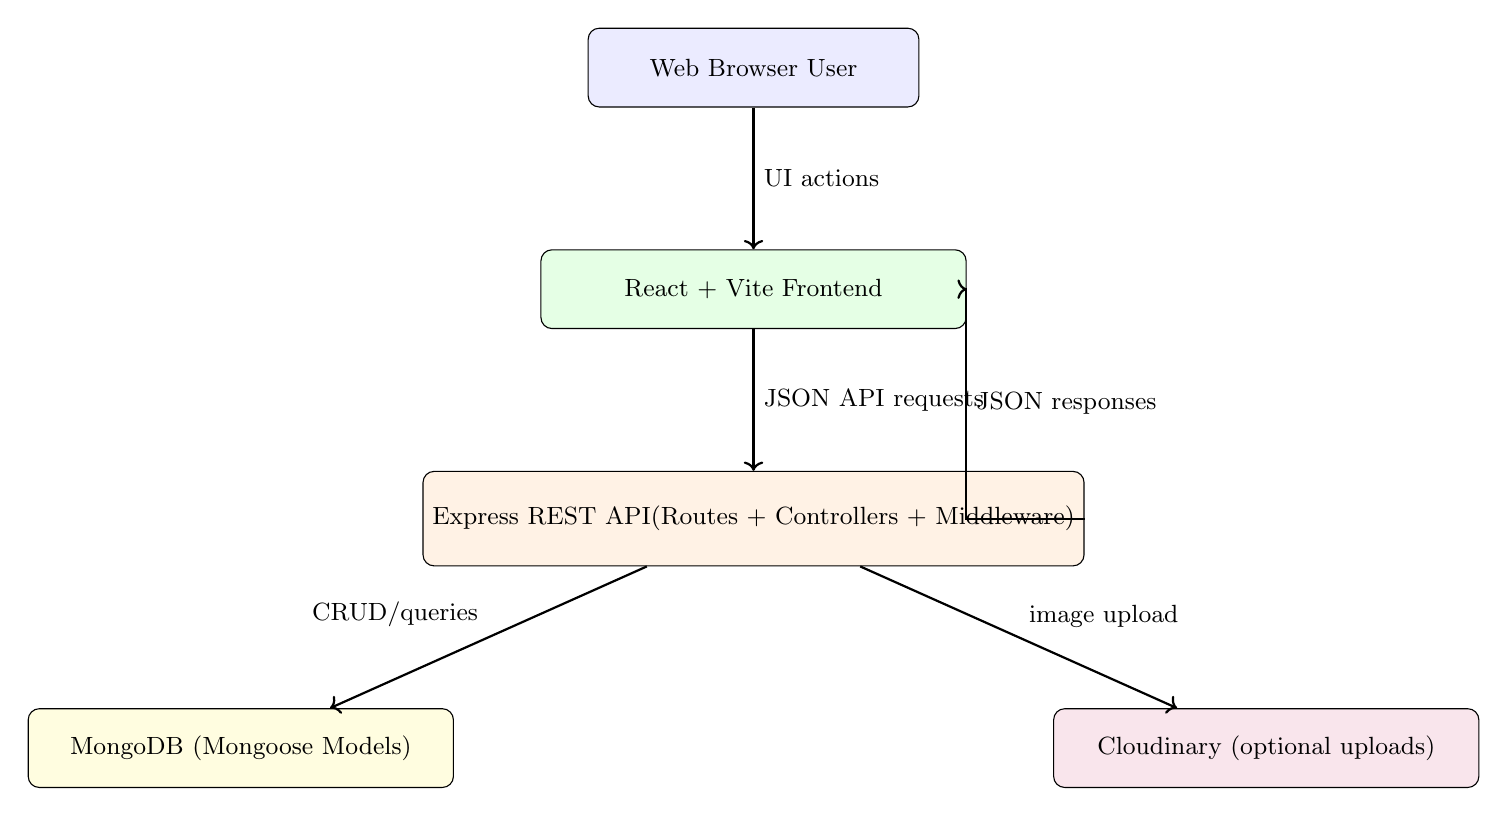
\begin{tikzpicture}[node distance=1.8cm, every node/.style={font=\small}]
    \node[draw, rounded corners, fill=blue!8, minimum width=4.2cm, minimum height=1cm] (client) {Web Browser User};
    \node[draw, rounded corners, fill=green!10, minimum width=5.4cm, minimum height=1cm, below=of client] (frontend) {React + Vite Frontend};
    \node[draw, rounded corners, fill=orange!10, minimum width=5.4cm, minimum height=1.2cm, below=of frontend] (api) {Express REST API\\(Routes + Controllers + Middleware)};
    \node[draw, rounded corners, fill=yellow!12, minimum width=5.4cm, minimum height=1cm, below left=1.8cm and -0.4cm of api] (db) {MongoDB (Mongoose Models)};
    \node[draw, rounded corners, fill=purple!10, minimum width=5.4cm, minimum height=1cm, below right=1.8cm and -0.4cm of api] (cloud) {Cloudinary (optional uploads)};

    \draw[->, thick] (client) -- node[right]{UI actions} (frontend);
    \draw[->, thick] (frontend) -- node[right]{JSON API requests} (api);
    \draw[->, thick] (api) -- node[above left]{CRUD/queries} (db);
    \draw[->, thick] (api) -- node[above right]{image upload} (cloud);
    \draw[->, thick] (api) -- ++(2.7,0) |- node[pos=0.25,right]{JSON responses} (frontend);
\end{tikzpicture}
\caption{High-level architecture of the Ebook Shop mini project}
\end{figure}

\section*{6.3 Request-Flow Summary}
Typical request flow is: user action on frontend page $\rightarrow$ context/helper triggers API request $\rightarrow$ Express route maps to controller $\rightarrow$ model operation on MongoDB $\rightarrow$ JSON response returned to frontend $\rightarrow$ UI state updated.

\chapter{Modules Description}
\section*{7.1 Authentication Module}
\textbf{Frontend:} Login and Register pages collect credentials, validate form fields, call API, and persist auth object in local storage.\\
\textbf{Backend:} Auth controller validates inputs, checks uniqueness, hashes password during registration, verifies password during login, and returns JWT token payload.

\section*{7.2 Book Catalog Module}
\textbf{Frontend:} Books context loads all books from backend and normalizes fields for UI presentation. Shop page supports search/filter/sort. Book Details page renders full information and related books.\\
\textbf{Backend:} Book controller supports list and single-book retrieval. Additional create/update/delete and upload endpoints exist.

\section*{7.3 Cart Module}
Cart module is client-side and stored in browser local storage. It supports add, remove, quantity increment/decrement, subtotal calculation, cart count, and clear cart. This module is active across pages through Cart Context provider.

\section*{7.4 Wishlist Module}
Wishlist is a hybrid module: UI interactions are in frontend, while persistence is in backend user document. Protected routes ensure only authenticated users can fetch or mutate wishlist entries.

\section*{7.5 Checkout and Order Module}
Checkout module validates billing inputs, computes payable amount (subtotal + tax + platform fee), and submits order payload to backend. Backend stores order document with order items, shipping address, payment method, and payment status flags.

\section*{7.6 Common UI and Navigation Module}
Reusable components (header, top bar, category strip, banner, cards, form controls, footer) provide consistent presentation and route navigation. The module improves maintainability by reducing repeated page markup.

\section*{7.7 Backend Infrastructure Module}
This module includes database connection configuration, JWT middleware (`protect`/`admin`), environment variable loading, and centralized server startup/error handling setup in `server.js`.

\chapter{Working / Workflow}
The implemented workflow is summarized below:
\begin{enumerate}[label=\arabic*.]
    \item User opens the application and lands on Home page with categories and featured/trending sections.
    \item User navigates to Shop page and applies search, category, price, rating, and sort options.
    \item User opens a selected book details page.
    \item User adds a book to cart and/or wishlist.
    \item If user selects wishlist operation without login, user is prompted to login.
    \item User registers or logs in through authentication pages.
    \item Authenticated user can persist wishlist items using backend APIs.
    \item User reviews cart, updates quantity, and proceeds to checkout.
    \item User enters billing details and selects a payment method option.
    \item Frontend submits order payload to protected backend route (`POST /api/orders`).
    \item Backend stores order record in MongoDB and returns order identifier.
    \item Frontend displays order success state and clears local cart.
\end{enumerate}

For unsupported paths (invalid route, unavailable book, empty cart, API failures), the UI displays explicit empty/error states.

\chapter{Database Design}
\section*{9.1 Database Approach}
The project uses MongoDB with Mongoose schema definitions. The practical entity set is \textbf{User}, \textbf{Book}, and \textbf{Order}. Wishlist is implemented as an array of referenced book IDs inside user records. Order items store denormalized snapshots (title, qty, price, image) and optional relation to book ID.

\section*{9.2 Entity Relationships}
\begin{itemize}
    \item One User can have many Orders.
    \item One User can have many wishlist Book references.
    \item One Order can contain many Order Items.
    \item Each Order Item may reference one Book.
\end{itemize}

\section*{9.3 Schema Details}
\subsection*{User Collection}
\begin{longtable}{>{\raggedright\arraybackslash}p{0.26\textwidth} >{\raggedright\arraybackslash}p{0.2\textwidth} >{\raggedright\arraybackslash}p{0.44\textwidth}}
\toprule
\textbf{Field} & \textbf{Type} & \textbf{Purpose} \\
\midrule
name & String & Display name of user \\
email & String (unique) & Login identity and contact field \\
password & String (hashed) & Stored secure password hash \\
isAdmin & Boolean (default false) & Role flag for admin-protected routes \\
wishlist & [ObjectId $\rightarrow$ Book] & Saved book references for later purchase \\
createdAt/updatedAt & Date & Automatic timestamps \\
\bottomrule
\end{longtable}

\subsection*{Book Collection}
\begin{longtable}{>{\raggedright\arraybackslash}p{0.26\textwidth} >{\raggedright\arraybackslash}p{0.2\textwidth} >{\raggedright\arraybackslash}p{0.44\textwidth}}
\toprule
\textbf{Field} & \textbf{Type} & \textbf{Purpose} \\
\midrule
title & String & Book title \\
author & String & Author name \\
price & Number & Selling price \\
image & String & Cover image URL \\
description & String & Detailed description text \\
category & String & Category label for browsing/filtering \\
stock & Number/String usage pattern & Availability value used in UI \\
pdfUrl & String & Ebook file URL (if available) \\
preview & String & Preview URL/text field \\
summary & String & Short summary used in UI \\
createdAt/updatedAt & Date & Automatic timestamps \\
\bottomrule
\end{longtable}

\subsection*{Order Collection}
\begin{longtable}{>{\raggedright\arraybackslash}p{0.26\textwidth} >{\raggedright\arraybackslash}p{0.2\textwidth} >{\raggedright\arraybackslash}p{0.44\textwidth}}
\toprule
\textbf{Field} & \textbf{Type} & \textbf{Purpose} \\
\midrule
user & ObjectId $\rightarrow$ User & Owner of order \\
orderItems & Array & Purchased item snapshots \\
orderItems.book & ObjectId $\rightarrow$ Book & Optional book reference \\
orderItems.qty & Number & Quantity per item \\
orderItems.price & Number & Unit price at order time \\
shippingAddress & Object & Address details captured at checkout \\
paymentMethod & String & Selected method (card/upi/wallet etc.) \\
paymentResult & Object & Status and metadata placeholders \\
totalPrice & Number & Total amount saved with order \\
isPaid & Boolean & Payment completion flag \\
paidAt & Date & Payment timestamp when marked paid \\
createdAt/updatedAt & Date & Automatic timestamps \\
\bottomrule
\end{longtable}

\section*{9.4 Design Observation}
The schema design is appropriate for mini-project scale. However, strict field validation and stronger type consistency can be improved in future (for example: `stock` representation and stricter required constraints).

\chapter{Input / Output Design}
\section*{10.1 Key Input Forms}
\begin{longtable}{>{\raggedright\arraybackslash}p{0.24\textwidth} >{\raggedright\arraybackslash}p{0.3\textwidth} >{\raggedright\arraybackslash}p{0.36\textwidth}}
\toprule
\textbf{Interface} & \textbf{Input Fields} & \textbf{Validation/Behavior} \\
\midrule
Register & name, email, password, confirmPassword & Required checks, email format validation, password length, password match \\
Login & email, password & Required checks, email format validation, backend credential verification \\
Search/Filter (Shop) & search text, category, max price, minimum rating, sort option & Dynamic filter and sort on client-side derived book list \\
Cart & quantity increment/decrement, remove item, clear cart & State recalculation and local storage persistence \\
Checkout & fullName, email, phone, address, city, state, zipCode, paymentMethod & Required field checks, email format check, login required for order API call \\
Wishlist actions & add/remove/toggle on book cards/details & Requires login; invokes protected backend routes \\
Contact (UI simulation) & name, email, message & Client-side validation with local success message only \\
\bottomrule
\end{longtable}

\section*{10.2 Key Outputs}
\begin{longtable}{>{\raggedright\arraybackslash}p{0.24\textwidth} >{\raggedright\arraybackslash}p{0.64\textwidth}}
\toprule
\textbf{Output Type} & \textbf{Description} \\
\midrule
Home output & Category cards, featured/trending lists, promotional cards, trust section, newsletter block \\
Shop output & Filtered and sorted book grid with result count and category/search context \\
Book details output & Cover, author/category/price, ratings, description, specification panel, related books \\
Cart output & Item-wise totals and overall order summary (subtotal, tax, fee, total) \\
Checkout output & Success message with generated order identifier on successful API response \\
Wishlist output & Persisted saved books for logged-in user with move-to-cart option \\
Backend output & JSON responses for API success/errors including messages and data payloads \\
\bottomrule
\end{longtable}

\section*{10.3 Error and Empty States}
The UI includes explicit states for conditions such as books-loading errors, no search results, empty cart/wishlist, missing route, and missing book ID match. Backend similarly returns status-based JSON for unauthorized access and missing records.

\chapter{Features Implemented}
\section*{11.1 Fully Implemented and Verified}
\begin{enumerate}[label=\arabic*.]
    \item Route-based multi-page frontend structure with reusable layout components.
    \item User registration and login connected to backend authentication APIs.
    \item JWT-based protected route handling for wishlist and order routes.
    \item Book catalog retrieval from MongoDB through `/api/books`.
    \item Shop search/filter/sort workflow in frontend.
    \item Cart management with local persistence.
    \item Wishlist management with backend persistence for authenticated users.
    \item Checkout form validation and order creation in backend database.
    \item MongoDB model definitions for User, Book, and Order.
    \item Optional image upload endpoint integrated with Cloudinary middleware.
\end{enumerate}

\section*{11.2 Partially Implemented / Infrastructure-Ready}
\begin{enumerate}[label=\arabic*.]
    \item Admin-related backend capabilities exist (admin middleware and all-orders route), but no frontend admin panel is implemented.
    \item Book create/update/delete and upload APIs exist, but no authenticated admin UI workflow is integrated on frontend.
    \item Payment status fields and mark-paid route exist, but full payment gateway lifecycle is not implemented.
    \item Contact/newsletter flows are frontend-only simulations without backend service integration.
\end{enumerate}

\chapter{Advantages and Limitations}
\section*{12.1 Advantages}
\begin{enumerate}[label=\arabic*.]
    \item Clear modular structure improves readability and learning value.
    \item Practical full-stack integration (frontend + backend + database) is achieved for core user flows.
    \item Context-based state management avoids excessive prop drilling.
    \item Error/empty states improve user understanding during failures.
    \item API and schema design are sufficient for mini-project demonstration and incremental extension.
\end{enumerate}

\section*{12.2 Limitations}
\begin{enumerate}[label=\arabic*.]
    \item Book write routes are currently not protected by admin middleware, which is a security limitation.
    \item No frontend admin dashboard for managing books/orders/users.
    \item No real payment gateway integration (only local method selection and status placeholders).
    \item No order-history page in frontend despite backend support for `GET /api/orders/my`.
    \item Digital asset delivery/reader flow for paid ebooks is not fully implemented.
    \item Some UI text still refers to ``frontend-only'' scope, which is inconsistent with current backend integration.
\end{enumerate}

\chapter{Future Scope}
The project can be extended in a structured manner without rewriting the current architecture.
\begin{enumerate}[label=\arabic*.]
    \item Implement role-based admin frontend dashboard for book and order management.
    \item Protect book create/update/delete/upload routes using `protect` + `admin` middleware.
    \item Add user profile and order-history pages integrated with existing order APIs.
    \item Integrate real payment gateway workflow and webhook-based payment status updates.
    \item Implement secure ebook download/read access controlled by successful paid orders.
    \item Add input validation library on backend and stricter schema-level constraints.
    \item Add pagination and server-side search/filter for large book datasets.
    \item Add automated test suites (unit/integration) for controllers and critical frontend flows.
    \item Containerize deployment and add CI pipeline for lint/build/test quality gates.
\end{enumerate}

\chapter{Conclusion}
Ebook Shop successfully demonstrates a meaningful full-stack mini-project for web technology learning. The implemented system combines React-based user experience with Express API services and MongoDB persistence for key ecommerce-like workflows, including authentication, catalog browsing, wishlist persistence, and order creation.

From an academic perspective, the project achieves its primary educational goals: modular code organization, API-driven architecture, frontend-backend integration, and practical database usage. At the same time, the current codebase reflects realistic development-stage limitations such as missing admin UI, incomplete payment integration, and some security hardening needs on book management routes.

Overall, the project forms a strong foundation for further enhancement and can be extended into a more complete production-style ebook platform through incremental, well-scoped improvements.

\chapter{References}
\begin{enumerate}[label=\arabic*.]
    \item React Documentation. \url{https://react.dev/}
    \item Vite Documentation. \url{https://vite.dev/}
    \item React Router Documentation. \url{https://reactrouter.com/}
    \item Node.js Documentation. \url{https://nodejs.org/en/docs}
    \item Express.js Documentation. \url{https://expressjs.com/}
    \item MongoDB Documentation. \url{https://www.mongodb.com/docs/}
    \item Mongoose Documentation. \url{https://mongoosejs.com/docs/}
    \item JSON Web Token (jsonwebtoken) Documentation. \url{https://github.com/auth0/node-jsonwebtoken}
    \item bcryptjs Package Documentation. \url{https://www.npmjs.com/package/bcryptjs}
    \item Multer Documentation. \url{https://github.com/expressjs/multer}
    \item Cloudinary Node SDK Documentation. \url{https://cloudinary.com/documentation/node_integration}
\end{enumerate}

\chapter{Appendix}
\section*{16.1 Folder Structure (Verified Snapshot)}
\begin{verbatim}
Ebook Shop/
|-- backend/
|   |-- config/
|   |   |-- cloudinary.js
|   |   `-- db.js
|   |-- controllers/
|   |   |-- authController.js
|   |   |-- bookController.js
|   |   |-- orderController.js
|   |   `-- userController.js
|   |-- middleware/
|   |   |-- authMiddleware.js
|   |   `-- uploadMIddleware.js
|   |-- models/
|   |   |-- Book.js
|   |   |-- Order.js
|   |   `-- User.js
|   |-- routes/
|   |   |-- authRoutes.js
|   |   |-- bookRoutes.js
|   |   |-- orderRoutes.js
|   |   `-- userRoutes.js
|   |-- utils/
|   |   `-- generateToken.js
|   |-- server.js
|   `-- package.json
|-- src/
|   |-- components/
|   |-- context/
|   |-- data/
|   |-- pages/
|   |-- utils/
|   |-- App.jsx
|   |-- main.jsx
|   `-- index.css
|-- public/
|-- package.json
`-- README.md
\end{verbatim}

\section*{16.2 Important Backend API Endpoints}
\begin{longtable}{>{\raggedright\arraybackslash}p{0.18\textwidth} >{\raggedright\arraybackslash}p{0.28\textwidth} >{\raggedright\arraybackslash}p{0.18\textwidth} >{\raggedright\arraybackslash}p{0.26\textwidth}}
\toprule
\textbf{Method} & \textbf{Endpoint} & \textbf{Access} & \textbf{Purpose} \\
\midrule
POST & /api/auth/register & Public & Register new user and return token \\
POST & /api/auth/login & Public & Authenticate user and return token \\
GET & /api/books & Public & Fetch all books \\
GET & /api/books/:id & Public & Fetch single book by ID \\
POST & /api/books & Public (current code) & Create a book record \\
PUT & /api/books/:id & Public (current code) & Update a book record \\
DELETE & /api/books/:id & Public (current code) & Delete a book record \\
POST & /api/books/upload & Public (current code) & Upload image through Cloudinary pipeline \\
GET & /api/users/wishlist & Protected & Fetch logged-in user wishlist \\
POST & /api/users/wishlist/:id & Protected & Add a book to wishlist \\
DELETE & /api/users/wishlist/:id & Protected & Remove a book from wishlist \\
POST & /api/orders & Protected & Create order \\
GET & /api/orders/my & Protected & Fetch current user's orders \\
GET & /api/orders/:id & Protected & Fetch order by ID \\
PUT & /api/orders/:id/pay & Protected & Mark order as paid \\
GET & /api/orders & Protected + Admin & Fetch all orders (admin scope) \\
\bottomrule
\end{longtable}

\section*{16.3 Important Frontend Pages and Contexts}
\begin{longtable}{>{\raggedright\arraybackslash}p{0.28\textwidth} >{\raggedright\arraybackslash}p{0.58\textwidth}}
\toprule
\textbf{File/Module} & \textbf{Responsibility} \\
\midrule
src/App.jsx & Main route declarations and layout wrapper \\
src/context/AuthContext.jsx & Login/register/logout and auth persistence \\
src/context/BooksContext.jsx & Book loading from backend and UI normalization \\
src/context/CartContext.jsx & Local cart storage and cart operations \\
src/context/WishlistContext.jsx & Auth-aware wishlist API integration \\
src/pages/Shop/Shop.jsx & Search/filter/sort listing workflow \\
src/pages/BookDetails/BookDetails.jsx & Book detail view, wishlist/cart actions \\
src/pages/Checkout/Checkout.jsx & Billing form, validation, order submission \\
src/pages/Login/Login.jsx & Login form and redirect behavior \\
src/pages/Register/Register.jsx & Registration form and account creation \\
src/pages/Wishlist/Wishlist.jsx & Wishlist listing and move-to-cart operation \\
\bottomrule
\end{longtable}

\section*{16.4 Screenshot Placeholders}
\begin{figure}[H]
\centering
\fbox{\parbox[c][5cm][c]{0.85\textwidth}{\centering Screenshot 1: Home Page}}
\caption{Home page interface}
\end{figure}

\begin{figure}[H]
\centering
\fbox{\parbox[c][5cm][c]{0.85\textwidth}{\centering Screenshot 2: Shop Page with Filters}}
\caption{Book listing with search/filter/sort}
\end{figure}

\begin{figure}[H]
\centering
\fbox{\parbox[c][5cm][c]{0.85\textwidth}{\centering Screenshot 3: Checkout Success}}
\caption{Order placement output screen}
\end{figure}

\end{document}
